\documentclass[a4paper]{article}
\usepackage[english]{babel}
\usepackage[utf8]{inputenc}
\usepackage{graphicx}

%Includes "References" in the table of contents

%Title, date an author of the document
\title{Charles W. Bachman}
\author{Caroline Liu}

%Begining of the document
\begin{document}

\maketitle

Charles W. Bachman, in full Charles William Bachman III, best known for his early work on developing database management systems, particularly the Integrated Data Store (IDS). He has played various roles in his prolonged career in the software engineering industry as developer, entrepreneur, architect and other numerous roles.
\bigbreak
After several years of working in various positions in different firms, he founded Bachman Information Systems\cite{histmuseam} which mainly served for graphical support to the creation and maintenance of Bachman Diagrams.


\section{Early Life and Education}
Charles William Bachman III was born in Manhattan, Kansas, December 11, 1924. His father was in the position of head coach for a college in the area, thought later bringing with him the family to East Lansing where he took up other coaching positions in different universities. In 1943, after attaining sufficient credits in high school, he went to for courses in Michigan State University.\cite{ebritannica} Shortly after graduating from high school, having accomplished the a year of course work of college also, Bachman joined the United States Army for approximately three years during World War II.
\bigbreak
After his discharge from the army, he returned to Michigan State University studying mechanical engineering, remarking his statement “I was never interested in anything else. I was always going to be an engineer.” \cite{interview}He then graduated with a bachelor's degree in mechanical engineering in 1948 and a subsequent masters degree from the University of Pennsylvania, where he also gained studies business, though not fully completed\cite{histmuseam}.
\section{Career}
Later on in the year following his graduation, Bachman took up a position in the engineering department of Dow Chemical Company in Midland Michigan, where he tackled engineering economics problems. In 1957 he was appointed first head of a new data-processing department. Bach pioneered the introduction to probability into the PERT scheduling that was employed by the company. During this time, he was also set to work on the SHARE 9PAC project for the IBM 709, though later in 1960 having he plans being backed down Dow and him subsequently leaving the company.
\bigbreak
Following his departure from Dow, he found a new job in General Electric in New York, where he made his great innovation, the Integrated Data Store (IDS). The company was them merged with Honeywell Information Systems Inc. and Bachman was required to further improve the company's IDS for their product line\cite{histmuseam}. During his period in the company, he also conceived the idea of Bachman diagrams that was used in database designing.
\bigbreak
He later moved on to Cullinane Database Systems Inc. where he continued to work on database systems. In 1983 he left the company to start up his own business whose concentration was towards the engineering of Bachman diagrams its generated database schemas.  
\section{Contributions}
\subsection{Integrated Data Store}
Bachman's main contribution was the IDS when he was working for General Electric. This system was a network database management system that was widely used in industry and greatly known for its efficiency, which served for the company's manufacture of a transaction-orientated operating system, the Manufacturing Information and Control System (MIACS). He developed a data-base oriented version of the BASIC programming language. The main component was to maximise the performance of the system with the limited hardware conditions at the time.
\bigbreak
The IDS was later enhanced for the GE-600 computer but its disclosure  made a huge breakthrough at the time as it was the first disk-based database management system used in production. This highly increased productivity as before the programs did not have the accessibility of retrieving and modifying a certain "database" but they had to I/O the data to the problem, but the MIACS allowed permanent storage of the data unless explicitly deleted of modified. The system allowed the integration of different kinds of data, keeping track of the information as it is modified. It was also a huge move that Bachman managed to store IDS and MIACS applications onto a computer with only the equivalent of 40 Kbytes of memory.The MIACS also incorporated a transaction-oriented operating system that accepted "problem control cards" with their associated data-cards until the dispatch of the computer to the program, placing them in a priority sequence subsequent to the prior solved problem. Problems associated were handled by the "problem controller", the IDS. The two combined dominated for a long period until their opponents came along.\cite{award, histmuseam}
\bigbreak
The IDS was basis for the IDS II and the Conference/Committee on Data System Languages Data Base Task Group standards\cite{ids}.Bachman pioneering innovations to database management sytems later lead him to gained the Turing Award in 1973 "for his outstanding contributions to database technology"\cite{award}.
\newpage
\subsection{Bachman Diagrams (ER Diagrams)}
Bachman's other contribution was towards ER diagrams to establish relationships between different entities and the flow of data internally:
\bigbreak
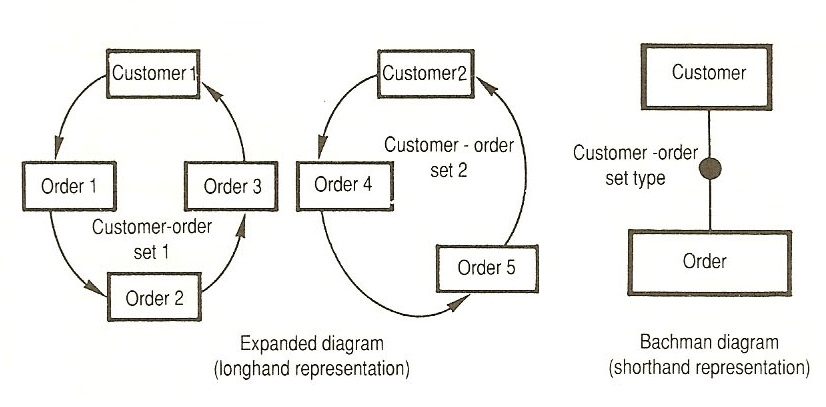
\includegraphics[scale=0.5]{Bachman_diagram.jpg}\cite{dig}
\bigbreak
In this type of model different entities are illustrated with rectangles which have a least one relational couple, that is, the arrow that connects the entities. On the edge of these arrows are the 1-to-1, 1-to-n or n-to-m cardinality of the relations.
\bigbreak
This is still commonly used in software design for the establishment and modelling of a specific database for a chosen system. Bachman himself also worked on building computer-aided software engineering (CASE) tools aids the engineering of such diagrams and forward and reverse generating of database schemas associated.
\section{Conclusion}
Bachman has without doubt, made great impact to  software engineering. With his determination to become a software engineer as a youngster, to his development of the IDS, setting groundbreaking milestones in the development of database management systems and the industry, his strong will is exceptional and inspiring to all.

%Sets the bibliography style to UNSRT and imports the 
%bibliography file "samples.bib".
\bibliographystyle{unsrt}
\bibliography{sample}

\end{document}
